\documentclass[12pt,UTF8]{ctexbook}
\usepackage{ctex}
\usepackage{array}
\usepackage{graphicx}
\usepackage{wrapfig}
\usepackage[table,dvipsnames]{xcolor}
\usepackage{tabularx}
\usepackage{amsmath}
\usepackage{amssymb}
\usepackage{xfrac}
\usepackage{eucal}
\usepackage{titlesec}
\usepackage{amsthm}
\usepackage{tikz-cd}
\usepackage{enumitem}
\usepackage{verbatim}
\usepackage{fontspec,xunicode,xltxtra}
\usepackage{xeCJK} 
\usepackage{caption}
\usepackage{thmtools, thm-restate}

\definecolor{gl}{RGB}{246, 252, 240}
\definecolor{gd}{RGB}{236, 244, 230}
\definecolor{bg}{RGB}{242, 244, 228}

\setCJKmainfont[BoldFont=STZhongsong]{STSong}
\setCJKmonofont{simkai.ttf} % for \texttt
\setCJKsansfont{simfang.ttf} % for \textsf
\setlength\parskip{8pt}
\setlength{\fboxsep}{12pt}
\renewcommand\thesection{\arabic{chapter}.\arabic{section}}
\newcommand{\arccot}{\operatorname{arccot}}
\newcommand{\dlim}[1]{^{\color{gray}\prime}#1}
\newcommand{\lian}[1]{
    \underset{#1}{\operatorname{lian}\,}
}
\newtheorem{df}{定义}[section] 
\newtheorem{pp}{命题}[section]
\newtheorem{tm}{定理}[section]
\newtheorem{ex}{例子}[section]
\newtheorem{et}{例题}[section]
\newtheorem{sk}{思考}[section]
\newtheorem*{po}{公理}
\newtheorem*{so}{解答}
\renewenvironment{proof}{\paragraph{\textbf{证明:}}}{\hfill$\square$}
\newtheorem{xt}{习题}[section]
\newtheorem{cor}{推论}[pp]

% 列举环境的行间距
\setenumerate[1]{itemsep=0pt,partopsep=0pt,parsep=0pt,topsep=0pt}
\setitemize[1]{itemsep=0pt,partopsep=0pt,parsep=0pt,topsep=0pt}
\setdescription{itemsep=0pt,partopsep=0pt,parsep=0pt,topsep=0pt}
% 章节字体大小
\titleformat{\section}{\zihao{-2}\bfseries}{ \thesection }{16pt}{}
% 封面
\title{\zihao{0} \bfseries 第三册}
\author{\zihao{2} \texttt{大青花鱼}}
% \date{\bfseries\today}
\date{}
% 正文
\begin{document}
\maketitle
\tableofcontents
\newpage

\chapter{无穷}
我们已经学习过无穷的概念。我们用数数原则来判定无穷。简单来说,数得尽的集合是有穷的,数不尽的集合是无穷的。
现在,我们来进一步探讨无穷的性质。

数数原则把集合分成有穷的和无穷的两种。有穷的集合,集合元素的个数是可以知道的,
因为按照定义,它是数得尽的。

我们把有穷集合的元素个数称为\textbf{集合的势},用数字绝对值的符号来表记。
比如,空集的势就是$0$,记作$|\varnothing| = 0$。集合$\{2,5,1\}$的势是$3$,
记作$|\{2, 5, 1\}| = 3$。

比较两个集合的势,可以用最简单的“对消法”:每次从集合$A$中“拿掉”一个元素,
对应地,也从集合$B$中“拿掉”一个元素。直到某个集合的元素被“拿光”。
如果另一个集合里还有元素,就说明前者的势小于后者;如果另一个集合里也没有元素了,就说明两者的势相等。

容易验证,有穷集合的势有以下的基本性质:
\begin{enumerate}
    \item 子集的势不多于母集的势;真子集的势小于真母集的势。
    \item 集合$A$在集合$B$中补集的势,加上$A$的势,等于$B$的势。
\end{enumerate}


\section{无穷集合的势}

有穷集合的基本性质符合我们日常生活中的经验。对于无穷集合,它们是否也成立呢?

来看以下的例子。

一个旅馆里有无穷个房间。房间的号码是正整数:$1$号、$2$号、$3$号……

一天,有一个客人来旅馆里住宿。可所有的房间都住了人,怎么办呢?
旅馆的老板说:这样吧,我们把$1$号房的客人转到$2$号房,把$2$号房的客人转到$3$号房,
把$3$号房的客人转到$4$号房……以此类推,$n$号房的人转到$n+1$号房。

这样,$1$号房就空出来了。客人顺利入住。

又一天,有无穷多个客人来旅馆里住宿。可所有的房间都住了人,怎么办呢?
旅馆的老板一看,每个客人有一个正整数号码,没有重复的也没有缺少的,恰好和房号一样。
老板说:这样吧,我们把$1$号房的客人转到$2$号房,把$2$号房的客人转到$4$号房,
把$3$号房的客人转到$6$号房……以此类推,$n$号房的人转到$2n$号房。

这样,所有奇数号的房间就空出来了。于是,$1$号客人住$1$号房,$2$号客人住$3$号房,$3$号客人住$5$号房,……以此类推,
$n$号客人入住$2n-1$号房。这样,所有的客人都顺利入住了。

以上的情况似乎有点违反我们的直觉。集合$\{2,3,4,\cdots\}$和$\{2,4,6,\cdots\}$是$\{1,2,3,\cdots\}$的真子集,
但它们的势与$\{1,2,3,\cdots\}$相等。这说明,无穷集合的势,有着不同的性质。

为此,我们首先要定义无穷集合的势的关系。我们从“对消法”出发来构思。
“对消法”中,我们实际上在给两个集合的元素建立一一对应的关系。
每次从两个集合里分别“拿掉”的元素形成一一对应。

如果一个集合“拿光”的时候,另一个集合也“拿光”了,
说明我们给两个集合的元素建立了一一对应的映射,也就是双射。

如果一个集合“拿光”的时候,另一个集合还有“剩余”,就说明我们无法在两个集合的元素之间建立双射。
我们可以从前一个集合出发,建立到后一个集合的单射;但无法从后一个集合出发,建立到前一个集合的单射。
这是因为后一个集合的元素太多了,总会有两个元素映射到同一个目标。

用这个思路,我们来定义无穷集合的势的关系。

\begin{df}\label{df:1-0-0}
    设有集合$A$和$B$。
    \begin{itemize}
        \item 如果存在$A$到$B$的双射,就说$A$和$B$的势相等,两者等势,记作$|A| = |B|$。
        \item 如果存在从$A$到$B$的单射,就说$A$的势不大于$B$的势或$A$的势小于等于$B$的势,记作$|A| \leqslant |B|$或$|B| \geqslant |A|$。
        \item 如果存在从$A$到$B$的单射,但不存在$B$到$A$的单射,就说$A$的势小于$B$的势,记作$|A| < |B|$或$|B| > |A|$。
    \end{itemize}
\end{df}

用这个定义,就可以理解无穷旅馆的例子。对于集合$\{1,2,3,\cdots\}$和$\{2,3,4,\cdots\}$来说,
我们有双射$n\mapsto n+1$,因此两者等势。
对于集合$\{1,2,3,\cdots\}$和$\{2,4,6,\cdots\}$来说,我们有双射$n\mapsto 2n$,因此两者等势。

注意:
\begin{enumerate}
    \item 以上定义对有穷集合、无穷集合都成立,也就是说,上面的$A$、$B$分别可以是有穷、无穷集合。
    \item 对于有穷集合$A$、$B$,这个定义与有穷集合的势的定义是兼容的。
    \item \textbf{无穷集合的势不是数}。我们沿用有穷集合的记法,把无穷集合$A$的势记作$|A|$。
    但$|A|$并不是任何数。因此,\textbf{无穷集合的势不能参与四则运算}。
    \item 同样地,当我们写$|A| \leqslant |B|$、$|A| = |B|$的时候,
    里面的等号和不等号也不能按数的相等、不等关系来理解。但在一定条件下,它们的性质和数的相等、不等关系是一样的(具体参见附录$A$)。
\end{enumerate}

\begin{sk}
    \mbox{} \\
    \indent 1. 在无穷旅馆的例子里,如果旅馆已经住满了,而有无穷多个旅客来住宿,
    旅客的编号用全体整数来编号。是否能腾出足够的房间呢?如何操作?如果旅客的编号用全体有理数呢?全体实数呢?\\
    \indent 2. 请用满射代替单射,定义无穷集合的势的关系。\\
    \indent 3. 能否给无穷集合的势定义四则运算?
\end{sk}


\begin{xt}
    \mbox{} \\
    \indent 1. 以下集合的势是多少?
    $$ 
    \begin{array}{l}
        1.\,1. \,\,\,\{\mbox{一年中的月份}\} \\
        1.\,2. \,\,\,\{100\mbox{以内的素数}\}\\
        1.\,3. \,\,\,\{S\mbox{的所有子集}\}\mbox{,其中}|S| = 9. \\
        1.\,4. \,\,\,\{(x, \,\, y, \,\, z) \, | \, 0 \leqslant x, y, z \leqslant 3, x + 2y + z \leqslant 8,\,\,\, x,\,\, y \in  \mathbb{Z}\}
    \end{array}
    $$
    \indent 2. 证明:把有穷集合的势定义为元素的个数,这样的定义,满足定义\ref{df:1-0-0} 中势的关系。\\
    \indent 3. 证明:有穷集合的势总小于无穷集合的势。\\
    \indent 4. 证明,如果集合$A$是$B$的子集,那么$|A| \leqslant |B|$。\\
    \indent 5. 证明:定义\ref{df:1-0-0} 中集合的势相等的关系,是一种等价关系,即满足:
    \indent \begin{itemize}
        \item 自反性:任意集合$A$的势等于自己:$|A| = |A|$。
        \item 对称性:若集合$A$的势等于集合$B$的势,则集合$B$的势等于集合$A$的势。
        \item 传递性:若集合$A$的势等于集合$B$的势,集合$B$的势等于集合$C$的势,则集合$A$的势等于集合$C$的势。
    \end{itemize}

    \indent 6. 证明:如果集合$A$、$B$满足$|A| < |B|$,那么$|A| = |B|$不成立。

    % \indent 6. 证明:定义\ref{df:1-0-0} 中集合的势小于等于的关系满足:\\
    % \indent \begin{itemize}
    %     \item 自反性:任意集合$A$的势等于自己:$|A| = |A|$。
    %     \item 对称性:任何集合$A$、$B$,$|A| \leqslant |B|$和$|B| \leqslant |A|$至少有一个成立。
    %     \item 传递性:若集合$A$的势小于等于集合$B$的势,集合$B$的势小于等于集合$C$的势,则集合$A$的势小于等于集合$C$的势。
    % \end{itemize}

    % \indent 7. 证明:定义\ref{df:1-0-0} 中集合的势小于的关系满足:
    % \indent \begin{itemize}
    %     \item 自背性:任意集合$A$的势不小于自己:$|A| < |A|$总不成立。
    %     \item 三分律:任何集合$A$、$B$的势总恰好满足$|A| < |B|$、$|A| = |B|$、$\qquad |B| < |A|$之一。
    %     \item 传递性:若集合$A$的势小于集合$B$的势,集合$B$的势小于集合$C$的势,则集合$A$的势小于集合$C$的势。
    % \end{itemize}
    
    
\end{xt}

\section{常见无穷集合的势}

常见的无穷集合有:自然数集$\mathbb{N}$、正整数集$\mathbb{Z}^+$、整数集$\mathbb{Z}$、
有理数集$\mathbb{Q}$、实数集$\mathbb{R}$等等。下面来看一些无穷集合的势的关系。

容易看出,$|\mathbb{N}| = |\mathbb{Z}^+|$,两者间的关系可以用双射$n\mapsto n + 1$确立。
而双射$n \mapsto -n$可以说明$|\mathbb{Z}^+| = |\mathbb{Z}^-|$,所以$|\mathbb{N}| = |\mathbb{Z}^-|$。

考虑把整数映射到自然数的映射:
$$ f,\,\,\,n\mapsto \left\{
    \begin{array}{cl}
        2n & \mbox{如果}n \geqslant 0 \\
        -2n - 1  & \mbox{如果}n < 0 
    \end{array}\right.
$$
也就是:
$$ \begin{array}{cccccccc}
        0 & -1 & 1 & -2 & 2 & -3 & 3 & \cdots \notag\\
        \downarrow & \,\downarrow & \downarrow & \,\downarrow & \downarrow & \,\downarrow & \downarrow & \cdots \notag\\
        0 & \,1 & 2 & \,3 & 4 & \,5 & 6 & \cdots \notag
    \end{array}
$$
它把所有自然数对应到自然数中的偶数,把所有负整数对应到自然数中的奇数。

不难验证,映射$f$是单射。
这是因为,给定两个不相同的正数$m \neq n$,如果两者一个小于零,一个不小于零,那么两者映射的结果奇偶性不同,因此不相等;
如果两者同时小于零或同时不小于零,按定义$2m \neq 2n$、$-2m - 1 \neq -2n - 1$,也就是说两者映射的结果不相等。
综上所述,如果$m \neq n$,那么$f(m) \neq f(n)$。

同时,映射$f$也是满射,因为任何偶数$n$都是整数$\frac{n}{2}$映射的结果,任何奇数$n$都是整数$-\frac{n+1}{2}$映射的结果。

$f$既是单射也是满射,因此是双射。我们在自然数集$\mathbb{N}$和整数集$\mathbb{Z}$之间建立了双射$f$,
这说明$|\mathbb{N}| = |\mathbb{Z}|$。

考虑平面所有坐标是自然数的点的集合:$\mathbb{N}^2 = \{(x,\,\,y) \, | \, x, \,\, y \in \,\, \mathbb{N}\}$。
$\mathbb{N}^2$的势与$\mathbb{N}$的势关系如何呢?

我们希望找出一种按顺序数出$\mathbb{N}^2$中所有点的数数方法。
这样,我们就可以把$1$映射到数数中的第一个点,把$2$映射到数数中的第二个点,等等,
建立从$\mathbb{Z}^+$到$\mathbb{N}^2$的映射。这个映射如果是双射,那么$\mathbb{N}^2$的势就等于$\mathbb{Z}^+$的势,从而等于$\mathbb{N}$的势。

考虑这样的数数方法:把点的横坐标和纵坐标加起来。从和最小的点开始数起,逐步增大。
对于和相等的点,则按照横坐标,从小数到大。
也就是按照图中箭头的方法来数数。这样的数法,可以不重复不遗漏地数遍$\mathbb{N}^2$所有的点。

\begin{figure}[h] %this figure will be at the right
    \vspace{4pt}
    \centering
    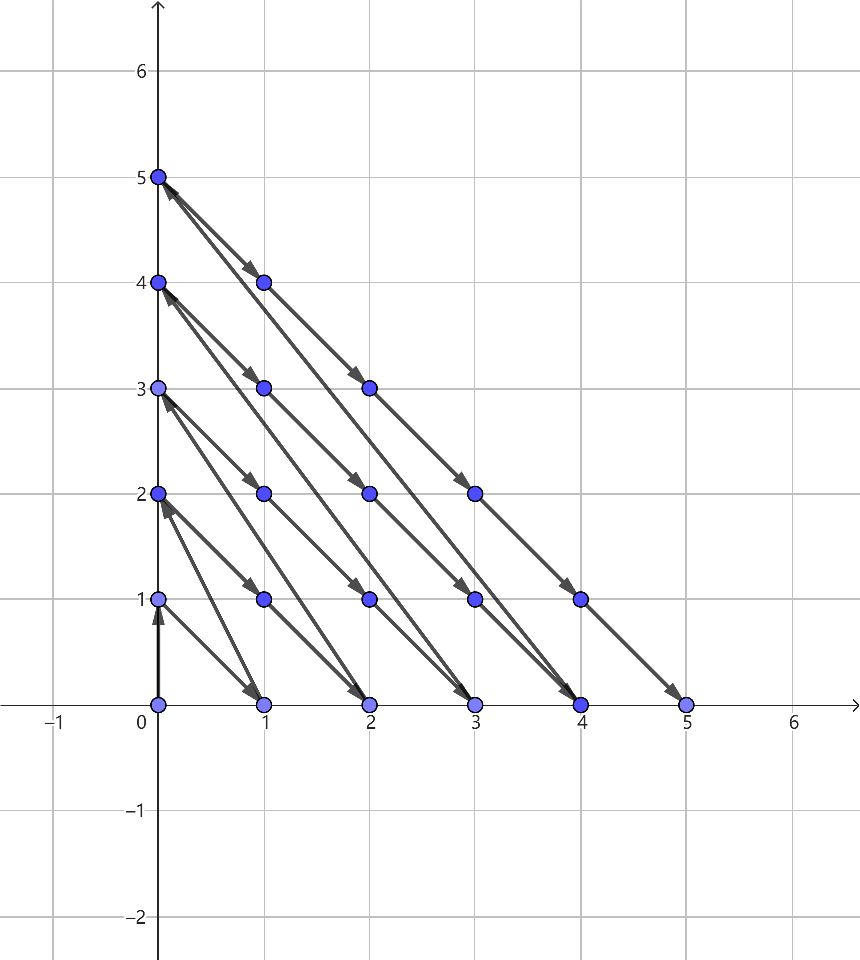
\includegraphics[width=0.4\textwidth]{无穷1.png}
    \caption*{\texttt{按照箭头方向,可以不重复不遗漏数遍}$\mathbb{N}^2$\texttt{中所有的点}}
\end{figure}

相应地,把正整数$n$映射到这个数法的第$n$个点,这样的映射就是双射。因此,按前面的推理,我们得到结论:
$$ |\mathbb{N}^2| = |\mathbb{N}|.$$

类似地,考虑正有理数集$\mathbb{Q}^+$。对有理数$r$,将它写成既约分数$\frac{p}{q}$,考虑分子分母之和。
从和最小的开始数起,逐步增加。如果某些有理数按以上方法得到的和相等,这样的有理数个数有限,把它们按分子从小到大排列,从分子最小的数起。
这样,我们得到了一种不重复不遗漏数遍所有正有理数的方法:
$$ \frac{1}{1} \rightarrow \frac{1}{2} \rightarrow \frac{2}{1} \rightarrow \frac{1}{3} \rightarrow \frac{3}{1} \rightarrow \frac{1}{4} \rightarrow \frac{2}{3} \rightarrow \frac{3}{2} \rightarrow \frac{4}{1} \rightarrow \cdots$$
这表明$\mathbb{Q}^+$的势等于$\mathbb{Z}^+$的势,从而等于$\mathbb{N}$的势。
$$ |\mathbb{Q}^+| = |\mathbb{N}|.$$

我们考虑把$\mathbb{N}$映射到$\mathbb{Q}^+$的双射$f$。考虑以下映射:
$$ g:\,\,\,r\mapsto \left\{
    \begin{array}{cl}
        0 & \mbox{如果}r = 0 \\
        f(r) & \mbox{如果}r > 0 \\
        -f(-r)  & \mbox{如果}r < 0 
    \end{array}\right.
$$
$g$把所有整数映射为有理数。由于$f$是双射,容易证明$g$也是双射。因此我们有$\mathbb{Z}$到$\mathbb{Q}$的双射,
这说明$\mathbb{Q}$的势等于$\mathbb{Z}$的势,从而等于$\mathbb{N}$的势。
$$ |\mathbb{Q}| = |\mathbb{N}|.$$

% \begin{sk}
%     \mbox{} \\
%     \indent 1. 
% \end{sk}


\begin{xt}
    \mbox{} \\
    \indent 1. 给定数集$A$和正整数$k\geqslant 2$,定义由$k$个$A$中元素构成的有序数组的集合为:
    $$ A^k = \{(a_1, a_2, \cdots, a_k) \, | \, a_1, a_2, \cdots, a_k \,\, \in A \}.$$
    \indent 1.1. 考虑$A = \mathbb{N}$的情况。考虑$\mathbb{N}^k$中的有序数组$(a_1, a_2, \cdots, a_k)$中的$k$个数的和。
    记所有和等于自然数$p$的有序数组构成的集合为$S_p$。证明:所有的$S_p$构成$\mathbb{N}^k$的分划。\\
    \indent 1.2. 给定正整数$k\geqslant 2$,考虑$\mathbb{N}^{k+1}$和$\mathbb{N}^{k}$按上一问构成的分划。
    如果$|\mathbb{N}^k| = |\mathbb{N}|$,证明:可以给出一种不重复不遗漏数遍$\mathbb{N}^{k+1}$的方法。\\
    \indent 1.3. 用归纳法证明:对任何正整数$k\geqslant 2$,$|\mathbb{N}^k| = |\mathbb{N}|$。\\
    \indent 1.4. 证明:$|\mathbb{Z}^k| = |\mathbb{N}|$。\\
    \indent 2. 证明:$\mathbb{N}$的子集要么有限,要么和$\mathbb{N}$等势。\\
    \indent 3. 证明:如果$|A| = |B| = |\mathbb{N}|$,那么$|A\cup B| = |\mathbb{N}|$。
\end{xt}

\section{可数和不可数}
上一节中,我们研究了一些常见数集的势。很多直观上似乎比自然数集“大得多”的数集,都和自然数集等势。
那么,是否有比自然数集“大”的数集呢?

考虑数列的项只有$0$和$1$的数列。我们把所有这样的数列构成的集合记为$2^\mathbb{N}$:
$$ 2^\mathbb{N} = \left\{\left\{a_n\right\}_{n\in\mathbb{N}} \, | \, \forall n\in\mathbb{N}, a_n \in \{0, 1\} \right\}. $$
下面我们证明:
$$|\mathbb{N}| < |2^\mathbb{N}|$$
也就是说,存在$\mathbb{N}$到$2^\mathbb{N}$的单射,但不存在$2^\mathbb{N}$到$\mathbb{N}$的单射。

首先考虑映射:
$$ \forall n\in\mathbb{N}, \quad n \mapsto \left\{a_k\right\}_{k\in\mathbb{N}}, \,\,\, \mbox{其中} \, a_k = 1 \,\mbox{当且仅当} \, k = n . $$
这个映射显然是单射,因此存在$\mathbb{N}$到$2^\mathbb{N}$的单射。

如何证明不存在$\mathbb{N}$到$2^\mathbb{N}$的单射呢?我们用反证法证明。

假设存在$2^\mathbb{N}$到$\mathbb{N}$的单射$f$,则$2^\mathbb{N}$所有元素经过映射得到的集合是$\mathbb{N}$的无穷子集,因而和$\mathbb{N}$等势。
也就是说,我们可以假设$f$是满射,因而是双射。因此,我们考虑它的逆映射$g$。$g$是把自然数映射到$2^\mathbb{N}$中元素的双射。
因此,我们可以把$2^\mathbb{N}$中的元素按数数的方式列出来:
\begin{align}
    0 &\mapsto a_{0,0}, a_{0,1}, a_{0,2}, \cdots , a_{0,k}, \cdots \notag \\
    1 &\mapsto a_{1,0}, a_{1,1}, a_{1,2}, \cdots , a_{1,k}, \cdots \notag \\
    2 &\mapsto a_{2,0}, a_{2,1}, a_{2,2}, \cdots , a_{2,k}, \cdots \notag \\
    \vdots & \qquad \qquad\qquad \vdots \notag \\
    n &\mapsto a_{n,0}, a_{n,1}, a_{n,2}, \cdots , a_{n,k}, \cdots \notag \\
    \vdots & \qquad \qquad\qquad \vdots \notag 
\end{align}
其中$a_{n,k}$是$n$对应的数列中的第$k$项。现在考虑这么一个数列$W$:
它的第$k$项就是$1$减去上面排列中$k$对应的数列的第$k$项。
也就是说,如果该项是$0$,$W$的第$k$项就是$1$,如果该项是$1$,$W$的第$k$项就是$0$。
按定义,$W$的第$k$项一定不等于上面排列中第$k$行数列的第$k$项。

按照$g$的定义,$W$肯定是某个自然数$m$经过$g$得到的结果,因此,它排在上面排列中的第$m$行。
但是,它的第$m$项就是$a_{m,m}$。然而按照$W$的定义,它的第$m$项应该是$1 - a_{m,m}$,不等于$a_{m,m}$。
这就构成了矛盾。

因此,不存在$\mathbb{N}$到$2^\mathbb{N}$的单射。

这样,我们得到了一个严格“大于”自然数集的集合。

以上结果说明:即便是无穷集合,也有“大小之分”。为此,我们要给无穷集合做更精细的划分。
注意到以上证明里,我们通过把$2^\mathbb{N}$中的元素用数数的方式列出来,而导出了矛盾。
这个矛盾说明了$2^\mathbb{N}$这样的集合的本质:它是“不可数”的。

我们把自然数集这样可以用数数的方式列出来的集合(也就是与$\mathbb{N}$等势的集合)
称为\textbf{可数集合}或\textbf{可列集合},
而把$2^\mathbb{N}$这样的集合称为\textbf{不可数集合}或\textbf{不可列集合}。
而以上的推理说明,\textbf{不可数集合总大于可数集合}。

不可数集合是否也有类似无限旅馆这样的现象呢?

对于可数集合,它的子集如果是无限的,就和它等势。
换句话说,如果从可数集合中去掉有限个元素,得到的子集和它等势。
用不严谨的话来说,这是由于有限集合相比可数集合是“非常小”的,是可以忽略的。

这个关系在可数集合与不可数集合之间也有体现。

\begin{tm}
    设$S$是不可数集合,它的子集$A$是可数集合,则$S$去除$A$中元素得到的集合$S\backslash A$与$S$等势。
\end{tm}

\begin{proof}
    首先用反证法证明$S\backslash A$是不可数集合。$S$是$A$与$S\backslash A$的并集。
    如果$A$和$S\backslash A$都是可数集合,那么它们的并集$S$也是可数集合。矛盾!

    接下来证明$|S\backslash A| = |S|$。考虑$S\backslash A$的可数子集$B$,记$S\backslash A$去掉$B$中元素得到的集合为$C$,
    则$A$、$B$、$C$是$S$的分划,$S = A\cup B\cup C$。
    
    注意到由于$S\backslash A$是不可数集合,$B$是可数集合,所以$C$也是不可数集合。
    另外,由于$A$、$B$是可数集合,所以$ |A| = |B| = |\mathbb{N}|$,于是$|A\cup B| = |\mathbf{N}|$。
    因此,存在从$B$到$A\cup B$的双射$g$。

    考虑映射:
    $$ f:\,\,\,x\mapsto \left\{
        \begin{array}{cl}
            g(x) & \mbox{如果}x\in B \\
            x & \mbox{如果}x \in C
        \end{array}\right.
    $$
    则$f$是$S\backslash A$到$S$的双射。因此$|S\backslash A| = |S|$。
    
\end{proof}

这说明,可数集合比起不可数集合,就和有限集合相比可数集合一样,是可以忽略的。

最后来看实数集$\mathbb{R}$。它是否可数呢?我们可以用证明$2^\mathbb{N}$类似的想法。

给定实数$x$,我们可以将它写成小数的形式。如果$x$是有穷小数,就在最后补上无穷多个$0$。
这样,每个实数都可以写成无穷小数。也就是说,我们可以把每个实数对应到类似$0$到$9$组成的无穷数列。

假设实数集可数,那么可以像前面的证明里那样,构造正整数集到实数集的双射,把所有实数依次排列出来。
各个实数的小数部分就和$2^\mathbb{N}$里的数列一样。于是,我们构造这样的实数$a$,
它的小数部分第$k$位数字和排第$k$位的实数的小数部分第$k$位数字不一样。
但另一方面,$a$也是某个正整数$m$映射的结果。因此按照定义,$a$的小数部分第$m$位不能等于自己。矛盾!
因此我们可以得出结论:实数集不可数。

实际上,我们可以严谨证明:实数集$\mathbb{R}$和$2^\mathbb{N}$等势,具体参见附录$A$。

研究了常见的无穷数集的势,我们发现,目前我们所知的无穷集合有两类。
一类数集与自然数集$\mathbb{N}$等势,是为可数集合。另一类与实数集$\mathbb{R}$等势,等于$2^\mathbb{N}$。
那么,是否有既不等势于$\mathbb{N}$,也不等势于$2^\mathbb{N}$的无穷集合呢?

数学研究者对无穷集合的研究发现:比$2^\mathbb{N}$“更大”的无穷集合是存在的。
我们把这些类别按从小到大的顺序,记为$\aleph_0$、$\aleph_1$、$\aleph_2$、$\aleph_3$等等。
$\aleph_0$就是自然数集$\mathbb{N}$,$\aleph_1$是$2^\mathbb{N}$。
$\aleph_2$、$\aleph_3$等则是比$2^\mathbb{N}$更大的集合。

另一方面,是否存在介于$\mathbb{N}$和$2^\mathbb{N}$之间的无穷集合,则是困难得多的问题。
由于实数集是连续的,我们把这个问题称为“连续统问题”或“连续统假设”。
对这个问题的研究直接引发了对数学基本推理框架的质疑。

1963年,数学家证明了:在我们常见的推理框架内,“连续统问题”是“独立的”,
既不可能证明它成立,也不可能证明它不成立。
从另一个角度来说,不论“存在介于$\mathbb{N}$和$2^\mathbb{N}$之间的无穷集合”还是
“不存在介于$\mathbb{N}$和$2^\mathbb{N}$之间的无穷集合”,都不会导致矛盾。

\begin{xt}
    \mbox{} \\
    \indent 1. 证明:可数集合去除有限个元素后仍然是可数集合。\\
    \indent 2. 证明:无理数集是不可数集合。\\
    \indent 3. 证明:可数个两两不相交的有限集合:$\{A_n\}_{n\in\mathbb{N}}$的并集是可数集合。\\
    \indent 4. 证明:有限个可数集合的并集是可数集合;可数个可数集合的并集是可数集合;不可数集合的并集是不可数集合。
\end{xt}

\chapter{连续函数的变化}

日常生活、工程和科学研究中,我们关心事物的运动和变化。
描述、衡量、分析事物的运动和变化,是人类了解世界、科学进步的关键。
17世纪,科学研究者发现了物体受力与运动变化的关系,建立了统一的力学理论,引发了工业革命。
20世纪初,科学研究者提出了“光速不变”的假设,在此基础上构建了相对论。
这些革命性的进步,都离不开对运动本质的探索。
而对运动的深入研究,也促使了数学的发展。

数学中,我们用实变映射描述事物的运动和变化。
具体来说,我们需要研究的事物性质一些基本要素相关。
这些基本要素,比如时间、物体的位置、温度等等,我们认为是连续变化的,称为变量,用实数表示。
于是,事物的性质就是关于这些变量的映射。
分析这些映射的性质,找到适合描述实验数据的映射,是科学研究的重要部分。

\section{函数在一点的变化}
% 介绍连续函数在一点的微变率:微变率是变化率的极限
我们已经学习过用数学描述运动和变化。对于物体的运动,我们定义了平均速度,描述运动的快慢。
一般来说,我们使用变率来描述事物变化的快慢。
\begin{df}{\textbf{实变映射的变率}}
    设$f$是定义在实数集上的映射,给定实数$t_1 < t_2$,则$f$在$[t_1,\,\,t_2]$上的\textbf{变率}是:
    $$ \frac{f(t_2) - f(t_1)}{t_2 - t_1}.$$
\end{df}

平均速度就是位移函数的变率。

使用平均速度,我们可以近似描述物体位置在一段时间里的变化。
如果把物体的运动看作关于时间$t$的函数,设物体的位移为函数$p(t)$,那么,在$(t_1, t_2)$的时间段里,
物体的位移大致是:
$$ p(t) \approx p(t_1) + \frac{p(t_2) - p(t_1)}{t_2 - t_1}(t - t_1).$$
这里我们用一次函数代替了真实的位移函数$p$。直观上,在区间$(t_1, t_2)$里,
我们用直线近似表示了函数$p(t)$的图像。

很多时候,我们希望对事物的变化有更好的理解。
比如,我们可以测量一秒内物体的位移,作为平均速度。但我们还想知道,如果把一秒换成更短的$0.1$秒、$0.01$秒,
得到的结果会不会完全不同。
此外,我们可以记录运动物体在某个时刻的位移,但也希望能记录物体在该时刻的速度(或者其他变化),
以更好地理解运动的性质。
甚至,我们发现物体受到的力与物体运动速度的变率相关,也就是说,和物体位移的变率的变率相关。
这时候,我们希望能更精确地知道物体运动速度的性质,以研究它的变率。
总之,我们需要一个刻画物体在某个时刻“附近”变化快慢的量。

实践中,我们发现,对于大多数的运动物体,如果在同样条件下重复测量平均速度,
那么随着取的时间间隔越来越短,测得的平均速度会趋于某个固定的值。这个现象让我们想到函数(在一点)的极限。
因此,我们用极限的概念来描述物体某个时刻“附近”变化的快慢。

我们可以定义物体在某个时刻$t_0$的瞬时速度$v(t_0)$:
$$ v(t_0) = \lian{t\to t_0} \frac{p(t) - p(t_0)}{t - t_0}.$$
它是$t$附近的平均速度的极限。正如数列的极限不一定等于数列自身的项,瞬时速度作为变率的极限,
描述了物体在该时刻运动的快慢,但它并非变率,也不是运动。

对于一般的函数,我们也可以用这个方法描述它在一点变化的快慢。

\begin{df}\label{df:2-0-0}
给定在某一点$a$附近有定义的函数$f$,如果当$x$趋于$a$时,
$f$在$a$到$x$的变率收敛到某个极限,就说函数$f$在$a$处\textbf{可微}。
我们把这个极限叫做函数$f$在点$a$处的\textbf{微变率},简称\textbf{微变},
记作$\partial f(a)$。\footnote{函数$f$在点$a$处的微变率,一般记作$\partial f(a)$或$f'(a)$,在物理书籍中也常记作$\dot{f}(a)$。
关于微变率的记法,可见附录$B$。}
$$ \partial f(a) = \lian{x\to a} \frac{f(x) - f(a)}{x - a} = \lian{h\to 0} \frac{f(a + h) - f(a)}{h}.$$
\end{df}

比如,运动物体在某时刻的瞬时速度,就是它的位移函数在该时刻的微变率。
$$ v(t_0) = \partial p(t_0).$$

\begin{figure}[h]
    \vspace{4pt}
    \centering
    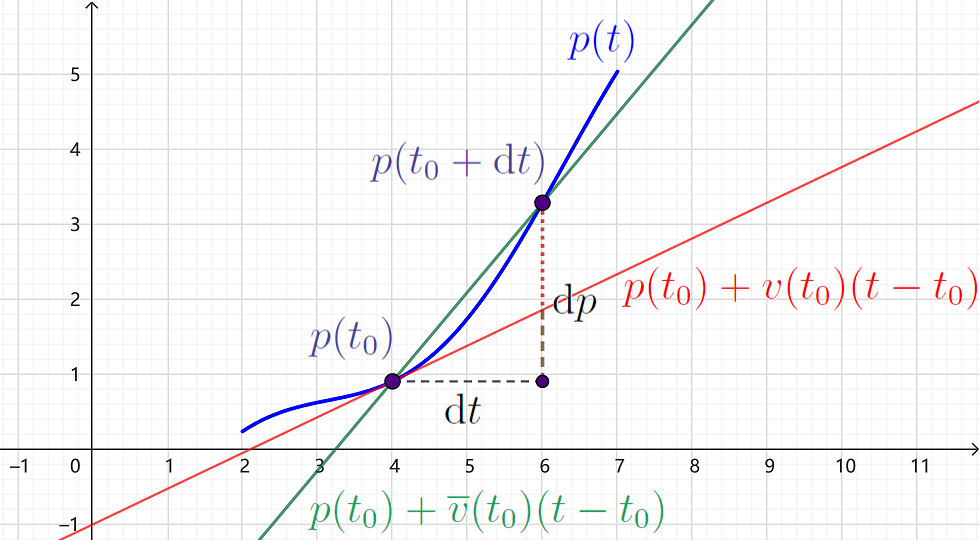
\includegraphics[width=0.7\textwidth]{导数1.png}
\end{figure}

如何理解瞬时速度呢?上图是物体做直线运动时,位移关于时间的函数的图像。横坐标表示时间$t$,
纵坐标表示物体的位移$p$。我们希望了解物体在$t_0$时刻“附近”的运动情况。

从$t_0$时刻起,经过固定时段$\mathrm{d}t$,
物体的位移产生了变化:
$$\mathrm{d}p = p(t_0 + \mathrm{d}t) - p(t_0).$$
因此,这段时间内的平均速度$\overline{v}(t_0)$就是$\mathrm{d}p$与$\mathrm{d}t$的比值:
$$\overline{v}(t_0) = \frac{\mathrm{d}p}{\mathrm{d}t}.$$
从图像来看,它是过函数两点构成的绿色直线的斜率。

使用平均速度,我们可以认为,在$t_0$附近,物体大致在做速度为$\overline{v}(t_0)$的匀速运动,
位移可以用一次函数近似表示:
$$ p(t) \approx p(t_0) + \overline{v}(t_0)(t - t_0)$$
直观来说,图中函数$p(t)$的图像曲线,在$t_0$附近,可以用绿色直线近似表示。

但是,要注意的是,平均速度$\overline{v}(t_0)$不仅仅与$t_0$相关。
对不同的$\mathrm{d}t$,$\overline{v}(t_0)$是不同的。而瞬时速度$v(t_0)$的存在告诉我们,
$\overline{v}(t_0)$会随着$\mathrm{d}t$缩小而收敛。
也就是说,绿色直线会逐渐收拢到过点$(t_0, \,\,p(t_0))$、以$v(t_0)$为斜率的红色直线。
我们称这条直线为函数图像在$t_0$的\textbf{切线}。

使用瞬时速度$v(t_0)$来近似描述$t_0$附近的运动,物体的位移可以用一次函数近似表示:
$$ p(t) \approx p(t_0) + v(t_0)(t - t_0).$$

这样的表示和之前有什么不同呢?

首先,我们注意到,瞬时速度$v(t_0)$只与$t_0$相关,不需要用别的时刻$t$来计算。
其次,我们可以证明,如果要用一次函数(也就是匀速运动)来近似表示物体在$t_0$附近的运动,
瞬时速度$v(t_0)$是“最好”的系数。

直观来说,如果用一条过$(t_0, \,\,p(t_0))$点的直线近似表示物体位移的曲线,
那么对于$t_0$附近的情况,斜率为$v(t_0)$的直线是“最好”的。

为什么这么说呢?

假设我们用某个数$u$做系数,用这样的一次函数:
$$ t \mapsto p(t_0) + u\cdot (t - t_0).$$
来近似表示物体的位移。考虑$t_0$附近的$t$,实际的位移是$p(t)$,近似的位移是$p(t_0) + u(t - t_0)$。
因此近似误差为:
$$ d(t) = \left|p(t) - p(t_0) - u(t - t_0)\right|. $$
这是一个关于$t$的函数。$t$趋于$0$时,$d(t)$趋于$0$。

让我们来研究它趋于$0$有多快。我们这样来衡量:以$t\mapsto t - t_0$为参照物,考虑$d(t)$和$|t - t_0|$的比值:
$$ \frac{d(t)}{|t - t_0|} = \left|\frac{p(t) - p(t_0) - u(t - t_0)}{t -  t_0}\right| =  \left|\frac{p(t) - p(t_0)}{t -  t_0} - u\right|. $$
如果这个比值在$t$趋于$t_0$的时候的极限是$0$,就说明只要$t$与$t_0$足够近,
近似误差$d(t)$就可以比$t-t_0$小得多。这就是说$d(t)$比$t-t_0$收敛得更快。
如果比值不趋于$0$,就说明$d(t)$并不比$t-t_0$收敛得更快。

考虑这个比值在$t$趋于$t_0$时的极限:
$$ \lian{t\to t_0} \frac{d(t)}{|t - t_0|} = \left|\lian{t\to t_0} \frac{p(t) - p(t_0)}{t -  t_0} - u\right| = |v(t_0) - u|. $$
因此,这个比值趋于$0$,当且仅当$v$等于瞬时速度$v(t_0)$。

换句话说,当且仅当$u = v(t_0)$时,近似误差$d(t)$比$t-t_0$收敛得更快。只要$t$与$t_0$足够近,
近似误差就可以比$t-t_0$小得多。而$v$取其他值的时候,就没有这样的效果,近似误差至多和$t-t_0$收敛得一样快。
也就是说,$u = v(t_0)$时,近似效果是最好的。
在$t_0$附近,用微变率作为系数的一次函数和原来的函数最像。
比如,我们取$t_0$处的瞬时速度$v(t_0)$作为$t_0$附近的“平均速度”,
就比取其他的平均速度更能表现$t_0$附近的运动。

一般来说,用微变率作为系数的一次函数:
$$ t \mapsto f(t_0) + \partial f(t_0) \cdot(t - t_0)$$
称为函数$f$在$t_0$处的\textbf{微直观}。
直观上,微直观就是函数$f$在$t_0$处的切线,是$t_0$附近模拟$f$图像曲线的最佳直线。

最后来看如何具体计算微变率。

从最简单的函数出发。
常函数$x \mapsto c$在任意点的微变都是$0$。
恒等函数$x\mapsto x$在任意点的微变都是$1$。
正比例函数$x \mapsto c x$在任意点的微变都是系数$c$。以上的结论就由读者来证明。

对于稍微复杂一点的函数,我们一起来算一算。

\begin{et}
    \mbox{} \\
    \indent 1. 求函数$f: \,\, x \mapsto x^2$在点$x = 3$处的微变率。\\
    \indent 2. 求函数$f: \,\, x \mapsto \frac{1}{x}$在点$x = 2$处的微变率。\\
    \indent 3. 求函数$f: \,\, x \mapsto (x - 1)^3$在点$x = 1$处的微变率。
\end{et}

\begin{so}
    \mbox{} \\
    \indent 1. 按定义,$f$在点$x = 3$处的微变率为:
    \begin{align}
        \partial f(3) &= \lian{h\to 0}\frac{f(3 + h) - f(3)}{h} \notag \\
        &= \lian{h\to 0}\frac{(3 + h)^2 - 3^2}{h} \notag \\
        &= \lian{h\to 0}\frac{6h + h^2}{h} \notag \\
        &= \lian{h\to 0}(6 + h) \notag \\
        &= 6.  \notag
    \end{align}

    \indent 2. 按定义,$f$在点$x = 2$处的微变率为:
    \begin{align}
        \partial f(2) &= \lian{h\to 0}\frac{f(2 + h) - f(2)}{h} \notag \\
        &= \lian{h\to 0}\frac{\frac{1}{2+h} - \frac{1}{2}}{h} \notag \\
        &= \lian{h\to 0}\frac{\frac{2 - (2 + h)}{2(2 + h)}}{h} \notag \\
        &= \lian{h\to 0}-\frac{1}{2(2 + h)} \notag \\
        &= -\frac{1}{2(2 + \lian{h\to 0}h)} \notag \\
        &= -\frac{1}{4}. \notag
    \end{align}

    \indent 3. 按定义,$f$在点$x = 1$处的微变率为:
    \begin{align}
        \partial f(2) &= \lian{h\to 0}\frac{f(1 + h) - f(1)}{h} \notag \\
        &= \lian{h\to 0}\frac{h^3 - 0}{h} \notag \\
        &= \lian{h\to 0}h^2 \notag \\
        &= 0. \notag
    \end{align}
\end{so}

\begin{sk}
    \mbox{} \\
    \indent 1. 在关于圆的章节中,我们定义:直线与圆恰有一个公共点,是为相切,公共点为切点。这个定义与本节中切线的定义相同吗?是否有矛盾的地方?\\
    \indent 2. 函数在一点可微,是否需要在该点有定义?是否需要在该点有极限?是否需要在该点连续?
\end{sk}

\begin{xt}
    \mbox{} \\
    \indent 1. 证明本节提到的关于常函数、恒等函数、正比例函数的微变率的结论。\\
    \indent 2. 求以下函数在给定点处的微变率。\\
    \indent 2.1. $f: \,\, x \mapsto x^4$在点$x = 2$处的微变率。\\
    \indent 2.2. $f: \,\, x \mapsto x^2 - 3x + 1$在点$x = 3$处的微变率。\\
    \indent 2.3. $f: \,\, x \mapsto \frac{1}{1 - 2x}$在点$x = -1$处的微变率。\\
    \indent 3. 已知函数$f$在$a$点可微,证明:函数$f$在$a$点连续。\\
    \indent 4. 我们这样定义函数$f$在$a$点\textbf{左可微}:函数$f$在$a$点左侧附近有定义。
    如果当$x<a$趋于$a$时,$f$从$a$到$x$的变率收敛到某个极限,就说函数$f$在$a$点左可微,
    称该极限为$f$在$a$点的\textbf{左微变率}或\textbf{左微变},记作:
    $$ \partial_- f(a) = \lian{x\to a^-} \frac{f(x) - f(a)}{x - a} = \lian{x\to a \\ x < a} \frac{f(x) - f(a)}{x - a}. $$
    \indent 4.1. 按照左可微的定义,定义\textbf{右可微}。\\
    \indent 4.2. 证明:函数$f$在$a$点可微,当且仅当它在$a$处左可微且右可微,且左右微变相等。
    这时$f$在$a$点的微变就是相等的左微变和右微变。\\
    \indent 4.3. 考虑绝对值函数:$f:x\mapsto |x|$。它在$0$处是否可微?
\end{xt}

\section{微变的运算法则}
% 函数经过加减乘除运算、复合函数、反函数的微变
已知函数的表达式,如何具体计算它在一点的微变率呢?与函数在一点的极限一样,
我们可以从研究最简单的函数的微变率开始,通过四则运算得到更复杂的函数的微变率。
为此,我们先来了解函数的运算与它(在一点的)微变的关系。

首先来看加减法。给定函数$f$、$g$和实数$a$。
设$f$、$g$在$a$处可微,微变率为$\partial f(a)$、$\partial g(a)$。
来看$f+g$、$f-g$在$a$处是否可导,为此,研究$f \pm g$变率的极限:
\begin{align}
    \lian{x\to a} \frac{(f \pm g)(x) - (f \pm g)(a)}{x - a} &= \lian{x\to a} \left(\frac{f(x) - f(a)}{x - a} \pm \frac{g(x) - g(a)}{x - a}\right) \notag \\
    &= \lian{x\to a} \frac{f(x) - f(a)}{x - a} \pm \lian{x\to a} \frac{g(x) - g(a)}{x - a} \notag \\
    &= \partial f(a) \pm \partial g(a) \notag
\end{align}
由此可见,$f+g$、$f-g$在$a$处也可微,微变率分别是$\partial f(a)$、$\partial g(a)$的和与差。
$$ \partial (f \pm g)(a) = \partial f(a) \pm \partial g(a) $$

接下来看乘法。同样地,研究$f \cdot g$变率的极限:
\begin{align}
    & \quad \lian{x\to a} \frac{(f \cdot g)(x) - (f \cdot g)(a)}{x - a} \notag \\
    &=  \lian{x\to a} \frac{f(x)\cdot g(x) - f(a)\cdot g(x) + f(a)\cdot g(x) - f(a)\cdot g(a)}{x - a} \notag \\
    &= \lian{x\to a} \left(g(x)\cdot\frac{f(x) - f(a)}{x - a} + f(a)\cdot\frac{g(x) - g(a)}{x - a}\right) \notag \\
    &= \lian{x\to a} g(x) \cdot \lian{x\to a}\frac{f(x) - f(a)}{x - a} + f(a)\cdot \lian{x\to a} \frac{g(x) - g(a)}{x - a} \notag \\
    &= g(a)\cdot\partial f(a) + f(a) \cdot\partial g(a) \notag
\end{align}
可以看到,$f \cdot g$在$a$处可微。不过,它的微变率并不是$\partial f(a)$、$\partial g(a)$的乘积。
$$ \partial (f \cdot g)(a) = g(a)\cdot\partial f(a) + f(a) \cdot\partial g(a) $$

再来看除法。研究$f \div g$变率的极限\footnote{和以往一样,为了让$f \div g$在$a$处有定义,这里需要假设$g(a)\neq 0$。}:
\begin{align}
    & \quad \lian{x\to a} \frac{(f \div g)(x) - (f \div g)(a)}{x - a} \quad = \quad \lian{x\to a} \frac{\frac{f(x)}{g(x)} - \frac{f(a)}{g(a)}}{x - a} \notag \\
    &= \lian{x\to a} \frac{1}{g(x)g(a)}\cdot\frac{f(x) g(a) - f(a) g(x)}{x - a} \notag \\
    &= \frac{1}{\lian{x\to a}g(x)g(a)} \cdot \lian{x\to a} \frac{f(x) g(a) - f(a) g(a) - (f(a) g(x) - f(a) g(a))}{x - a} \notag \\
    &= \frac{1}{g(a)^2}\cdot \left( g(a)\cdot \lian{x\to a} \frac{f(x) - f(a)}{x - a} - f(a) \cdot\lian{x\to a} \frac{g(x) - g(a)}{x - a}\right) \notag \\
    &= \frac{g(a)\cdot \partial f(a) - f(a)\cdot \partial g(a)}{g(a)^2} \notag
\end{align}
可以看到,$f \div g$在$a$处可微。不过,和函数乘法一样,
它的微变率并不是$\partial f(a)$除以$\partial g(a)$的商。
$$ \partial (f \div g)(a) = \frac{g(a)\cdot \partial f(a) - f(a)\cdot \partial g(a)}{g(a)^2} $$

综上可见,函数的四则运算的微变,并不是简单地把函数的微变作四则运算。
下面来看更复杂一点的,复合函数的微变率。

设$f$、$g$是定义在实数集上的函数,$a$为实数。$g$在$a$处可微,微变率为$\partial g(a)$;
$f$在$g(a)$处可微,微变率为$\partial f(g(a))$。
那么复合函数$f\circ g$是否在$a$处可微呢?

来看$f\circ g$在$a$处变率的极限:
\begin{align}
    & \quad \lian{x\to a} \frac{(f \circ g)(x) - (f \circ g)(a)}{x - a} \notag \\
    &= \lian{x\to a} \left(\frac{f(g(x)) - f(g(a))}{x - a} \cdot \frac{g(x) - g(a)}{g(x) - g(a)}\right) \notag \\
    &= \lian{x\to a} \frac{f(g(x)) - f(g(a))}{g(x) - g(a)} \cdot \lian{x\to a} \frac{g(x) - g(a)}{x - a} \notag \\
    &= \partial f(g(a)) \cdot \partial g(a) \notag \\
\end{align}
上面推导中,我们从$\lian{x\to a} \frac{f(g(x)) - f(g(a))}{g(x) - g(a)}$算出$\partial f(g(a))$,
是因为$g$在$a$处可微,从而连续,因此$x$趋于$a$时,$g(x)$趋于$g(a)$。因此,把$g(x)$整体看作变化量,
\begin{align}
    \lian{x\to a} \frac{f(g(x)) - f(g(a))}{g(x) - g(a)} &= \lian{t\to g(a)} \frac{f(t) - f(g(a))}{t - g(a)} \notag \\
    &= \partial f(g(a)) \notag 
\end{align}
综上,复合函数$f\circ g$在$a$处可微,微变率为:
$$ \partial (f\circ g) (a) = \partial f(g(a)) \cdot \partial g(a)$$
如果是多个函数的复合,比如三个函数$f$、$g$、$h$,那么可以算出,上式变为:
$$ \partial (f\circ g \circ h) (a) = \partial f(g(h(a))) \cdot \partial g(h(a)) \cdot h(a).$$
多次复合的微变是各次复合的微变的乘积,仿佛链条一样。这个结果被形象地称为“\textbf{链式法则}”。

最后来看反函数的微变率。设$f$是定义在实数集上的函数,$a$为实数,$f$在$a$处可微,微变率为$\partial g(a)$。
$f$在$a$附近有反函数$g$,即对$a$附近的$x$,总有$f(g(x)) = g(f(x)) = x$。$g(f(a)) = a$。
那么反函数$g$在$f(a)$处是否可微呢?

假设$g$在$a$处可微。考虑$f\circ g$,它是恒等函数,恒等函数在任意点的微变率是$1$。因此,根据链式法则,我们有:
$$ 1 = \partial (g\circ f) (a) = \partial g(f(a)) \cdot \partial f(a)$$
也就是说,
$$ \partial g(f(a)) = \frac{1}{\partial f(a)} $$
$g$在$f(a)$处的微变率是$\partial f(a)$的倒数。这要求$\partial f(a)$不能为零。

假设$\partial f(a)$不为零,计算$g$在$f(a)$处变率的极限:
\begin{align}
    & \quad \lian{x\to f(a)} \frac{g(x) - g(f(a))}{x - f(a)} \notag \\
    &= \lian{x\to f(a)} \frac{g(x) - a}{x - f(a)} \notag \\
    &= \lian{g(x)\to a} \frac{g(x) - a}{f(g(x)) - f(a)} \notag \\
    &= \frac{1}{\lian{g(x)\to a}\frac{f(g(x)) - f(a)}{g(x) - a}} \notag \\
    &= \frac{1}{\partial f(a)} \notag
\end{align}
上面推导中,我们用到了反函数的连续性:$f$在$a$处连续,因此$g$在$f(a)$处连续。因此$x$趋于$f(a)$时,
$g(x)$趋于$g(f(a))$,也就是$a$。

\begin{et}
    \mbox{} \\
    \indent 1. 求以下函数在给定点处的微变率。\\
    \indent 1.1. $f: \,\, x \mapsto (x + 1)(3x -4)$在点$x = 2$处的微变率。\\
    \indent 1.2. $f: \,\, x \mapsto \frac{x - 1}{2x^2 - x + 1}$在点$x = 1$处的微变率。\\
    \indent 1.3. $f: \,\, x \mapsto (2x - 1)^3$在点$x = -1$处的微变率。\\
\end{et}

\begin{so}
    \mbox{} \\
    \indent 1. 应用函数乘法的求微法则:
    \begin{align}
        \partial f(2) &= \partial (x + 1) (2) \cdot (3 \cdot 2 - 4) + \partial (3x - 4) (2) \cdot (2 + 1) \notag \\
        &= 1 \cdot (3 \cdot 2 - 4) + 3 \cdot (2 + 1) \notag \\
        &= 6 + 9 = 15 \notag  
    \end{align}
    其中$\partial (x + 1) (2)$表示函数$x\mapsto x + 1$在$x = 2$处的微变率。$\partial (3x - 4) (2)$同理。\\
    \indent 2. 应用函数除法的求微法则:
    \begin{align}
        \partial f(1) &= \frac{\partial (x - 1) (1) \cdot (2 \cdot 1^2 - 1 + 1) - \partial (2x^2 - x + 1) (1) \cdot (1 - 1)}{(2\cdot 1^2 - 1 + 1)^2} \notag \\
        &= \frac{ 1 \cdot 2 - 3 \cdot 0}{2^2} \notag \\
        &= \frac{1}{2} \notag  
    \end{align}
    \indent 3. 应用复合函数的求微法则(链式法则):
    \begin{align}
        \partial f(-1) &= \partial (x^3) (2\cdot (-1) - 1) \cdot \partial (2x - 1) (-1) \notag \\
        &= 3\cdot (-3)^2 \cdot 2 \notag \\
        &= 54 \notag  
    \end{align}

\end{so}

\begin{sk}
    \mbox{} \\
    \indent 1. 在函数的除法和反函数的求微法则中,都有要求取值不为零的情况。
    请对应函数图像,给出这些要求的直观解释。\\
    \indent 2. 对比函数在一点的极限,函数在一点微变率的运算法则有什么不同?你觉得为什么会有这样的不同。\\
    \indent 3. 对于把实数变量映射到向量的映射,能否定义在某个实数$t$的微变率?如何在直观上解释你定义的微变率?\\
    \indent 4. 对于把向量映射到向量的映射,也就是点映射,能否定义在某个点的微变率?如何在直观上解释你定义的微变率?
    
\end{sk}

\begin{xt}
    \mbox{} \\
    \indent 1. 求以下函数在给定点处的微变率。\\
    \indent 1.1. $f: \,\, x \mapsto (2x - 1)(x -4)(x^2 + 3)$在点$x = 2$处的微变率。\\
    \indent 1.2. $f: \,\, x \mapsto \frac{(x + 1)(x^2 + 1)}{x^3 - 2x + 3}$在点$x = 1$处的微变率。\\
    \indent 1.3. $f: \,\, x \mapsto (2x - \frac{1}{x + 1})^5$在点$x = 0$处的微变率。\\
    \indent 2. 函数$x \mapsto x^{\frac{1}{3}}$在$x = 0$处是否可微?\\
    \indent 3. 考虑以下函数:
    $$ f: \,\,\, x\mapsto \left\{
        \begin{array}{cl}
            x & \mbox{如果}x\mbox{为有理数} \\
            -x & \mbox{如果}x\mbox{为无理数} 
        \end{array}\right.
    $$
    \indent 3.1. 证明:$f$在$x = 0$处可微。\\
    \indent 3.2. 证明:$f$在$x = 1$处不可微。\\
    \indent 3.3. 找出$f$所有可微的点,并给出证明。
\end{xt}

\section{常见函数的微变}

使用上一节中的结论,我们来研究一些较为复杂的常见函数的微变。

首先来看整式函数的微变。给定整式:$a_0 + a_1 x + a_2 x^2 + \cdots + a_n x^n$,其中$a_0, a_1, \cdots , a_n$是整式的系数。
它是一系列单项式$x^k$乘以系数后相加的结果。因此,我们可以先研究形如$x^k$的单项式。

给定自然数$k$,$x\mapsto x^k$是$k$个$x$的乘积。对于$k=0$、$k=1$的情况,我们已经知道对应的微变:
$$ \forall \,\, a, \quad \partial (x^0) (a) = 0, \quad \partial (x^1) (a) = 1 $$
$k > 1$时,根据函数乘法的求微法则,
$$ \partial (x^{k+1}) (a) = \partial (x^{k} \cdot x) (a) = \partial (x^k) (a) \cdot a + 1 \cdot a^k. $$
用归纳法可以证明:
$$ \forall k \in \mathbb{Z}^+, \,\,\, a\in \mathbb{R}, \quad \partial (x^k) (a) = k a^{k-1}. $$
因此,我们可以得出一般整式函数的微变:
$$ \forall a, \quad \partial (a_0 + a_1 x + a_2 x^2 + \cdots + a_n x^n) = a_1 + 2 a_2 x + \cdots + n a_n a^{n-1}. $$

接下来看幂函数$x^r$的微变。
对自然数$k$,函数$x \mapsto x^{\frac{1}{k}}$是单项式函数$x\mapsto x^k$的反函数,所以根据反函数的求微法则:
\begin{align}
    \partial (x^{\frac{1}{k}}) (a) &= \frac{1}{\partial (x^k) (a^{\frac{1}{k}})} \notag \\
    &= \frac{1}{k a^{\frac{k-1}{k}}} \notag \\
    &= \frac{1}{k} a^{\frac{1}{k} - 1} \notag
\end{align}
要注意的是,这里用到了反函数的求微法则,所以,根据对应的要求,$a$不能为$0$。
$a = 0$时,函数不可微。

对于$r = \frac{p}{q}$为非零有理数时,函数$x \mapsto x^r$可以看作函数$x \mapsto x^{\frac{1}{q}}$与函数$x \mapsto x^{p}$的复合函数,
因此,根据复合函数的求微法则:
\begin{align}
    \partial (x^{\frac{p}{q}}) (a) &= \partial (x^p) (a^{\frac{1}{q}}) \cdot \partial (x^{\frac{1}{q}}) (a) \notag \\
    &= p \cdot a^{\frac{p - 1}{q}} \cdot \frac{1}{q} \cdot a^{\frac{1}{q} - 1} \notag \\
    &= \frac{p}{q} a^{\frac{p}{q} - 1} \notag    
\end{align}
综上可知,对非零有理数$r$,如果函数$x \mapsto x^r$在一点$a$附近有定义,那么其微变为:
$$ \partial (x^r) (a) = r a^{r-1}. $$
要注意的是,“在一点$a$附近有定义”的要求是必需的,它包括了$a \neq 0$的要求。

再来看三角函数的微变。我们需要用到之前的结论:
$$ \lian{x\to 0} \frac{\sin{x}}{x} = 1.$$

对于正弦函数$\sin$,计算变率的极限:
\begin{align}
    \partial \sin(a) &= \lian{h\to 0} \frac{\sin{a + h} - \sin{a}}{h} \notag \\
    &= \lian{h\to 0} \frac{\sin{a}\cos{h} + \cos{a}\sin{h} - \sin{a}}{h} \notag \\
    &= \sin{a} \lian{h\to 0} \frac{\cos{h} - 1}{h} + \cos{a} \lian{h\to 0}\frac{\sin{h}}{h} \notag \\
\end{align}
这里我们要计算两个极限,第二个极限可以直接使用上面的结论,结果是$1$。
对于第一个极限,我们把分子转化为关于$\sin$的表达式。
\begin{align}
    \lian{h\to 0} \frac{\cos{h} - 1}{h} &= \lian{h\to 0} \frac{\cos^2{h} - 1}{h(\cos{h} + 1)} \notag \\
    &= \lian{h\to 0} -\frac{\sin{h}}{h} \cdot \lian{h\to 0} \frac{\sin{h}}{\cos{h} + 1} \notag \\
    &= -1 \cdot \frac{0}{1 + 1} \notag \\
    &= 0.
\end{align}
因此,正弦函数$\sin$在一点$a$的微变为:
$$ \partial \sin(a) = \cos{a} $$

类似地,可以计算余弦函数$\cos$的微变。变率的极限:
\begin{align}
    \partial \cos(a) &= \lian{h\to 0} \frac{\cos{a + h} - \cos{a}}{h} \notag \\
    &= \lian{h\to 0} \frac{\cos{a}\cos{h} - \sin{a}\sin{h} - \cos{a}}{h} \notag \\
    &= \cos{a} \lian{h\to 0} \frac{\cos{h} - 1}{h} - \sin{a} \lian{h\to 0}\frac{\sin{h}}{h} \notag \\
    &= \cos{a} \cdot 0 - \sin{a} \cdot 1 = -\sin{a} \notag
\end{align}
余弦函数$\cos$在一点$a$的微变为:
$$ \partial \cos(a) = -\sin{a} $$

正切函数$\tan$可以看作正弦函数和余弦函数的比值,因此,它在一点$a$的微变为:
\begin{align}
    \partial \tan(a) &= \partial \left(\frac{\sin{a}}{\cos{a}}\right) \notag \\
    &= (\frac{\partial \sin(a) \cdot \cos{a} - \partial \cos(a) \cdot \sin{a}}{\cos^2{a}} \notag \\
    &= \frac{\cos^2{a} + \sin^2{a}}{\cos^2{a}} \notag \\
    &= \frac{1}{\cos^2{a}}. \notag 
\end{align}
正切函数$\cos$在一点$a$的微变为:
$$ \partial \tan(a) = \frac{1}{\cos^2{a}} $$

余切$\cot$是正切的倒数,使用求微法则可知,余切函数在一点$a$的微变为:
$$ \partial \cot(a) = -\frac{1}{\sin^2{a}} $$

最后来看指数函数。给定底数$c > 1$,指数函数$x\mapsto c^x$是连续函数,计算它在一点$a$的微变:
\begin{align}
    \partial (c^x) (a) &= \lian{h\to 0} \frac{c^{a+h} - c^a}{h} \notag \\
    &= c^a \lian{h\to 0} \frac{c^h - 1}{h} \notag \\
    &= c^a \cdot \partial (c^x) (0) \notag
\end{align}
可以看到,如果指数函数在$0$处可微,那么它在任意点处可微,且微变率是函数值与函数在$0$处微变率的乘积。

于是,我们来研究指数函数在$0$处的微变。对于不同的底数$c_1$、$c_2$,有:
$$c_2^h = c_1^{\frac{log{c_2}}{\log{c_1}}\cdot h}.$$
因此,
\begin{align}
    \lian{h\to 0} \frac{c_2^h - 1}{h} &= \lian{h\to 0} \frac{c_1^{\frac{log{c_2}}{\log{c_1}}\cdot h} - 1}{h} \notag \\
    &= \frac{log{c_2}}{\log{c_1}} \cdot \lian{h\to 0} \frac{c_1^{\frac{log{c_2}}{\log{c_1}}\cdot h} - 1}{\frac{log{c_2}}{\log{c_1}} \cdot h} \notag \\
    &= \frac{log{c_2}}{\log{c_1}} \cdot \lian{t\to 0} \frac{c_1^{t} - 1}{t} \notag 
\end{align}
也就是说,如果底数$c_1$的指数函数在$0$处可微,那么底数$c_2$的指数函数在$0$处也可微,并且两个微变率只差一个乘法系数。

考虑通项公式如下的数列$\{e_n\}$:
$$ \forall n\in\mathbb{Z}^+,\quad e_n = \left(1 + \frac{1}{n}\right)^n.$$
可以证明,数列$\{e_n\}$有极限$e$。而$e$满足:
$$ \lian{t\to 0} \frac{e^{t} - 1}{t} = 1.$$
因此,对任意底数$c$,指数函数$x\mapsto c^x$在$0$处可微,微变率是:
$$ \lian{h\to 0} \frac{c^h - 1}{h} = \log_e{c}.$$
从而,指数函数$x\mapsto c^x$在$a$处的微变率为:
$$ \partial (c^x) (a) = c^a \cdot \log_e{c}. $$

指数函数在任一点的微变率与它在该点的值成正比,比值是以$e$为底数的对数$\log_e{c}$。

特别来说,以$e$为底数时,指数函数$f: x\mapsto e^x$在任一点的微变率等于它在该点的值。
$$ \partial f (a) = e^a = f(a).$$

对数函数是指数函数的反函数。因此,可以用反函数的求微法则,求出对数函数的微变。
\begin{align}
    \partial log_c (a) &= \frac{1}{\partial (c^x) (log_c{a})} \notag \\
    &= \frac{1}{a \cdot log_e{c}} \notag 
\end{align}
对数函数在定义域中任一点的微变率与它在该点的值成反比,比值是以$e$为底数的对数$\log_e{c}$的倒数。

同样,如果底数为$e$,那么对数函数在任一点的微变率等于它在该点的值的倒数。
$$ \partial \log_e (a) = \frac{1}{a}.$$
为此,我们把以$e$为底数的对数函数称为\textbf{自然对数},记作$\ln$。而$e$也叫做\textbf{自然对数的底数}。

\begin{et}
    \mbox{} \\
    \indent 1. 求以下函数在给定点处的微变率。\\
    \indent 1.1. $f: \,\, x \mapsto \sin{(2x - 7)}$在点$x = 2$处的微变率。\\
    \indent 1.2. $f: \,\, x \mapsto \log_2{\left(\frac{x+1}{x-1} + \sin(x)\right)}$在点$x = 2$处的微变率。\\
    \indent 1.3. $f: \,\, x \mapsto 3^{2x - \frac{1}{\sin{x} + 2}}$在点$x = -1$处的微变率。\\
\end{et}

\begin{so}
    \mbox{} \\
    \indent 1. 应用复合函数的求微法则:
    \begin{align}
        \partial f(2) &= \partial \sin (2 \cdot 2 - 7) \cdot \partial (2x - 7) (2) \notag \\
        &= \cos{(-3)} \cdot 2 \notag \\
        &= 2 \cos{3} \notag  
    \end{align}
    
    \indent 2. 应用复合函数的求微法则:
    \begin{align}
        \partial f(2) &= \partial \log_2 \left(\frac{2+1}{2-1} + \sin{2}\right) \cdot \left(\partial \left(\frac{x+1}{x-1}\right) (2) + \partial \sin (2) \right)\notag \\
        &= \frac{1}{\log_e{2} \left(\frac{2+1}{2-1} + \sin{2}\right)} \cdot \left( -\frac{2}{(2 - 1)^2} + \cos{2} \right) \notag \\
        &= \frac{\cos{(2)} - 2}{\ln{2} \cdot (3 + \sin{2})} \notag  
    \end{align}
    \indent 3. 应用复合函数的求微法则:
    \begin{align}
        \partial f(-1) &= \partial (3^x) (2\cdot (-1) - \frac{1}{2 + \sin{-1}}) \cdot \left(\partial (2x) (-1) - \partial \frac{1}{\sin{x} + 2} (-1) \right) \notag \\
        &= \ln{3} \cdot 3^{-2 - \frac{1}{2 - \sin{1}}} \cdot \left(2 - \frac{-1}{(\sin{(-1)} + 2)^2} \cdot \cos{(-1)} \right) \notag \\
        &= \frac{\ln{3}}{3^{2 + \frac{1}{2 - \sin{1}}}} \cdot \left(2 + \frac{\cos{1}}{(2 - \sin{1})^2}\right) \notag 
    \end{align}

\end{so}

\begin{sk}
    \mbox{} \\
    \indent 1. 有理函数在哪些地方可微?哪些地方不可微?\\
    \indent 2. \\
    \indent 3. 对于把实数变量映射到向量的映射,能否定义在某个实数$t$的微变率?如何在直观上解释你定义的微变率?\\
    \indent 4. 对于把向量映射到向量的映射,也就是点映射,能否定义在某个点的微变率?如何在直观上解释你定义的微变率?
    
\end{sk}

\begin{xt}
    \mbox{} \\
    \indent 1. 求以下函数在给定点处的微变率。\\
    \indent 1.1. $f: \,\, x \mapsto (2x - 1)(x -4)(x^2 + 3)$在点$x = 2$处的微变率。\\
    \indent 1.2. $f: \,\, x \mapsto \frac{(x + 1)(x^2 + 1)}{x^3 - 2x + 3}$在点$x = 1$处的微变率。\\
    \indent 1.3. $f: \,\, x \mapsto (2x - \frac{1}{x + 1})^5$在点$x = 0$处的微变率。\\
    \indent 2. 函数$x \mapsto x^{\frac{1}{3}}$在$x = 0$处是否可微?\\
    \indent 3. 考虑以下函数:
    $$ f: \,\,\, x\mapsto \left\{
        \begin{array}{cl}
            x & \mbox{如果}x\mbox{为有理数} \\
            -x & \mbox{如果}x\mbox{为无理数} 
        \end{array}\right.
    $$
    \indent 3.1. 证明:$f$在$x = 0$处可微。\\
    \indent 3.2. 证明:$f$在$x = 1$处不可微。\\
    \indent 3.3. 找出$f$所有可微的点,并给出证明。
\end{xt}





\section{微变函数的性质}
% 中值定理
\section{多次微变}
% 多次微变,k阶光滑

\chapter{研究函数}
\section{增减与极值}
% 一阶微变
\section{凹凸性质}
% 凸函数,琴声不等式,拐点
\section{局部性质}
% 高阶无穷小、泰勒公式
\section{曲线的性质}
% 参数方程曲线的局部性质研究

\chapter{平直空间}
%将平面和立体空间扩展为一般的平直空间
\section{平直空间的基本性质}
\section{子空间与和空间}
\section{生成空间}
\section{基底和维数}

\chapter{连续函数的和}
\section{函数图像的面积}
\section{函数的定合}
\section{合函数}

\chapter{级数}
\section{正项级数}
\section{收敛与发散}
\section{函数的级数}



\begin{appendix}

\chapter{序、序数和集合的势}

\begin{tm}
    实数集$\mathbb{R}$和$2^\mathbb{N}$等势。
\end{tm}

\begin{proof}
    直接建立$\mathbb{R}$和$2^\mathbb{N}$之间的双射,比较困难。我们使用区间$(0,1)$作为“中介”。
    首先建立$(0,1)$到$\mathbb{R}$的双射$f_1$,然后建立$2^\mathbb{N}$到$(0,1)$的双射$f_2$。
    这样,$f_1$和$f_2$的复合就是$2^\mathbb{N}$到$\mathbb{R}$的双射。
    
    首先建立$(0,1)$到$\mathbb{R}$的双射。考虑反三角函数$\arccos$在$(-1,1)$上的取值,
    它把$(-1,1)$上的数映射到$(0,\pi)$上,是从$(-1,1)$到$(0,\pi)$的双射。
    而余切函数$\cot$则是从$(0,\pi)$到$\mathbb{R}$的双射。因此映射
    $$ f_1 :\quad x \mapsto \cot{\left(\arccos{(2x-1)}\right)} $$
    是从$(0,1)$到$\mathbb{R}$的双射。

    再来把区间$(0,1)$的实数和$2^\mathbb{N}$联系起来。
    考虑$2^\mathbb{N}$中的数列$\{a_n\}_{n\in\mathbb{N}}$。

    取数轴上区间$[0,1]$的中点$0.5$,它把$[0,1]$平分成两个区间。
    如果$a_0 = 0$,就取左边的区间$[0,0.5]$,否则取右边的区间$[0.5,1]$。
    然后在新的闭区间里,根据$a_1$的值重复上一步的操作。
    这样不断下去,得到一个闭区间套。根据闭区间套定理,它趋于某个$[0,1]$中的实数。

    如果数列从某一项后全是$0$或全是$1$,那么从某一步操作后我们将总是取左边(右边)的区间。
    这样闭区间套会收敛到这一步对应的区间的左(右)端点,它对应着某个分母是$2$的乘方的有理数。
    除此以外,区间套收敛到某个$(0,1)$中的实数。这个实数不是分母是$2$的乘方的有理数。

    把$2^\mathbb{N}$中所有从某一项后全是$0$或全是$1$的数列的集合记为$A$,
    把$(0,1)$中所有分母是$2$的乘方的有理数的集合记为$B$,那么以上的操作构造了从
    $2^\mathbb{N}\backslash A$到$(0,1)\backslash B$的映射$g_1$。

    下面证明$g_1$是双射。

    首先证明$g_1$是单射。给定$2^\mathbb{N}\backslash A$中两个不同的数列,设它们最早从第$k$项起不同,
    那么对应的第$k$步操作时就会选择同一区间$[a,b]$的左部分$[a,\frac{a+b}{2}]$和右部分$[\frac{a+b}{2},b]$。而由于数列不会从某一项后全是$0$或全是$1$,
    所以最终闭区间套不会收敛到端点上,也就是说两者经过$f$映射的结果分别在$(a,\frac{a+b}{2})$和$(\frac{a+b}{2},b)$中,因此不相等。

    再证明$g_1$是满射。$\forall x \in (0,1)\backslash B$,用以下操作构建数列$\{a_n\}$:
    取数轴上区间$[0,1]$的中点$0.5$,它把$[0,1]$平分成两个区间。
    如果$x<0.5$,则$a_0=0$,取左边的区间;否则$a_0=1$,取右边的区间。
    然后在新的区间里重复上一步的操作,决定$a_1$的值。以此类推,得到数列$\{a_n\}\in 2^\mathbb{N}$。

    以上操作同样得到一个闭区间套,且收敛到$\{x\}$。由于$x\notin B$,
    所以不会有从某次操作后总是取左边(右边)的区间的情况,也就是说,得到的数列不在$A$中。
    这就说明$x$必然是$2^\mathbb{N}\backslash A$中某个数列经过$g_1$映射的结果,也就是说,$g_1$是满射。
    
    $g_1$既是单射又是满射,因此是双射。

    另一方面,考虑集合$A$和$B$。我们来建立$A$和$B$之间的双射。
    
    $B$是有理数集的无穷子集,因此是可数集合。
    而集合$A$可以作以下分划:

    设$k$为自然数,记$A_k$为所有最早自$a_k$起全是$0$或全是$1$的数列的集合。所有$A_k$两两不相交,
    且并集是$A$。

    计算它们的势。$|A_0| = |A_1| = 2$,
    $$ \forall \,\, k > 1, \quad |A_k| = 2^{k-1}. $$
    因此,$A_0$、$A_1$和$\{0,1,2,3\}$一一对应;$k>1$时,每个$A_k$和$\{2^{k-1}+3,2^{k-1}+4,\ldots, 2^k+2\}$一一对应。
    于是$A$和自然数集一一对应。

    于是,存在$A$到$B$的双射$g_2$。这样,我们就可以构造$2^\mathbb{N}$到区间$(0,1)$的双射$f_2$:
    $$ f_2:\,\,\,x\mapsto \left\{
        \begin{array}{cl}
            g_1(x) & \mbox{如果}x \in 2^\mathbb{N}\backslash A \\
            g_2(x) & \mbox{如果}x \in A 
        \end{array}\right.
    $$

    把$f_1$和$f_2$复合,我们就完成了$\mathbb{R}$和$2^\mathbb{N}$之间双射关系的构造。
    结论:
    $$ |\mathbb{R}| = |2^\mathbb{N}|. $$

\end{proof}

\chapter{微变与求合}

\section{函数的微变与微变的函数}
\begin{tm}{\textbf{直指不等式}}\label{tm:b2-0-20}
    设有正整数$n > 1$,实数$x > -1$且$x \neq 0$,则$(1 + x)^n > 1 + nx.$
\end{tm}

\begin{proof}
    用归纳法证明。$n = 1$时有$(1 + x)^n = 1 + nx$。假设对正整数$n$有$(1 + x)^n \geqslant 1 + nx$,
    下面证明$(1 + x)^{n+1} > 1 + (n+1)x$。
    \begin{align}
        (1 + x)^{n+1} &= (1 + x)^{n} \cdot (1 + x) \notag \\
        &\geqslant (1 + nx)(1 + x) \notag \\
        &= 1 + (n + 1)x + nx^2 \notag \\
        &> 1 + (n + 1)x.
   \end{align}
   因此,由$n=1$的情况可以推出$n=2$时$(1 + x)^{2} > 1 + 2x$。
   此后对所有$n>2$,总有$(1 + x)^{n} > 1 + nx$。
\end{proof}

\begin{tm}\label{tm:b2-0-30}
    对任意正整数$k$,数列$\{\left(1 + \frac{k}{n}\right)^n\}_{n\in\mathbb{Z}^+}$收敛。
\end{tm}

\begin{proof}
    记数列$\{u_{k,n}\}_{n\in\mathbb{Z}^+}$、$\{v_{k,n}\}_{n\in\mathbb{Z}^+}$的通项分别是:
    $$
    \forall n \in\mathbb{Z}^+, \quad
    \begin{array}{cl}
        u_{k,n} &=  \left(1 + \frac{k}{n}\right)^n, \\
        v_{k,n} &= \left(1 + \frac{k}{n}\right)^{n+1}.
    \end{array}
    $$
    只要证明$\{u_{k,n}\}$是单调递增数列,$\{v_{k,n}\}$是单调递减数列。
    那么$\{u_{k,n}\}$、$\{v_{k,n}\}$都是有界数列,因而都有极限,
    分别记为$u_{k}, v_k$。

    又注意到对任意正整数$n$,
    $$v_{k,n} - u_{k,n} = \frac{k}{n} \cdot u_{k,n}, $$
    因此差数列$\{v_{k,n} - u_{k,n}\}$收敛到$0$。所以$u_k = v_k$。
    我们定义$e = u_1 = v_1$。

    下面证明$\{u_{k,n}\}$是单调递增数列。

    对任意正整数$n$:
    \begin{align}
        \frac{u_{k,n+1}}{u_{k,n}} &= \frac{\left(1 + \frac{k}{n+1}\right)^{n+1}}{\left(1 + \frac{k}{n}\right)^n} \notag \\
        &= \frac{\left(1 + \frac{k}{n+1}\right)^{n+1}}{\left(1 + \frac{k}{n}\right)^{n+1}} \cdot \left(1 + \frac{k}{n}\right) \notag \\
        &= \left(\frac{n(n+k+1)}{(n+1)(n+k)}\right)^{n+1} \cdot \left(1 + \frac{k}{n}\right) \notag \\
        &= \left(1 + \frac{-k}{(n+1)(n+k)}\right)^{n+1} \cdot \left(1 + \frac{k}{n}\right) \notag \\
        &> \left(1 + \frac{-k}{n+k}\right)\cdot \left(1 + \frac{k}{n}\right) \notag \\
        &= 1 \notag 
    \end{align}
    其中的不等号根据直指不等式(\ref{tm:b2-0-20})可得。注意:由于直指不等式对任意$x>-1$且$x\neq 0$成立,
    所以只要$k$是非零实数,对于足够大的$n$,不等号总成立。也就是说,对非零实数$k$,
    数列$\{\left(1 + \frac{k}{n}\right)^n\}_{n\in\mathbb{Z}^+}$在$n$足够大的时候总是单调递增数列。

    再证明$\{v_{k,n}\}$是单调递减数列。对任意正整数$n$,考虑均值不等式:
    $$ \frac{(n+1)\cdot \frac{1}{n+1} + k\cdot \frac{1}{n}}{n+k+1} > \left(\left(\frac{1}{n+1}\right)^{n+1} \cdot \left(\frac{1}{n}\right)^{k}\right)^{\frac{1}{n+k+1}} $$
    据此可以得到:
    $$ \left(1 + \frac{k}{n}\right)^{n+k+1} > \frac{(n+k+1)^{n+k+1}}{(n+1)^{n+1} n^k}. $$
    因此,
    \begin{align}
        \left(1 + \frac{k}{n}\right)^{n+1} &> \frac{(n+k+1)^{n+k+1}\cdot n^k}{(n+1)^{n+1}\cdot n^k\cdot (n+k)^k} \notag \\
        &= \left(1 + \frac{k}{n+1}\right)^{n+2} \cdot \frac{(n+1)(n+k+1)^{k-1}}{(n+k)^k} \notag
    \end{align}
    只需证明$\frac{(n+1)(n+k+1)^{k-1}}{(n+k)^k} > 1$,就得到$v_{k,n} > v_{k,n+1}$。
    
    而这个不等式等价于:
    $$ \left(1 + \frac{1}{n+1}\right)^{k-1} > \frac{n+k}{n+1} = 1 + \frac{k-1}{n+1}.$$
    根据直指不等式,上式成立。于是我们证明了$\{v_{k,n}\}$是单调递减数列。
\end{proof}

对非零有理数$r = \frac{p}{q}$,注意到
$$ \left(1 + \frac{r}{n}\right)^n = \left(1 + \frac{p}{qn}\right)^n = u_{p,qn}^\frac{1}{q}$$
于是数列$\{u_{r,n}\} = \{\left(1 + \frac{r}{n}\right)^n\}_{n\in\mathbb{Z}^+}$其实就是
数列$\{u_{p,n}^{\frac{1}{q}}\}$的子列,因而收敛。

\begin{tm}\label{tm:b2-0-40}
    对任意有理数$r$,数列$\{\left(1 + \frac{r}{n}\right)^n\}_{n\in\mathbb{Z}^+}$收敛。
\end{tm}

考虑关于$x$的函数$f_{n} : x \mapsto \left(1 + \frac{x}{n}\right)^n $。
对足够大的正整数$n$,$1 + \frac{x}{n} > 0$, 于是$f_n$对于$x$总是单调递增函数。所以只要$a < b$,
对足够大的正整数$n$就有$u_{a,n} < u_{b,n}$。因此它们对应的数列的极限$u_a$、$u_b$就有$u_a \leqslant u_b$。
也就是说,定义在有理数上的函数:
$$ h: \,\,\, r \mapsto \lian{n\to\infty}  \left(1 + \frac{r}{n}\right)^n $$
单调递增。

对于函数$h$,我们还知道什么呢?首先容易验证:
$$ h(0) = 1, \quad h(1) = e.$$ 
从此不难做出这样的猜想:
$$ h(x) = e^x. $$

对正整数$k$,考虑$u_{k,kn}$:
$$ u_{k,kn} = \left(1 + \frac{k}{kn}\right)^{kn} = \left(1 + \frac{1}{n}\right)^{kn}, $$
因此,当$n$趋于无穷时,数列$\{u_{k,kn}\}$趋于$h(1)^k$。而它又是$\{u_{k,n}\}$的子列,
所以趋于$h(k)$。这说明$h(k) = e^k$。

考虑$u_{1,kn}$,它等于$u_{\frac{1}{k},n}^k$,所以$\{u_{\frac{1}{k},n}\}$趋于$h(1)^{\frac{1}{k}}$,
即$h(\frac{1}{k}) = e^{\frac{1}{k}}$。

同理,对于有理数$r = \frac{p}{q}$,考虑$u_{p,qn}$,
它等于$u_{\frac{p}{q},n}^q$,所以$\{u_{\frac{p}{q},n}\}$趋于$h(p)^{\frac{1}{q}}$,也就是$h(1)^{\frac{p}{q}}$。
这说明$h(r) = e^{\frac{p}{q}}$。

综上可知,对任何有理数$r$,$h(r) = e^r$。

给定实数$x$,选择任意有理数$r^{\text{下}} < x < r^{\text{上}}$,则$n$足够大时,
$u_{r^\text{下},n} < u_{x,n} < u_{r^\text{上},n}$。
因此,数列$\{u_{x,n}\}$有界且单调递增,因此收敛。

我们把它的极限定为$h(x)$,就把$h$的定义域扩延到了实数集上。

使用第一册中探索指数函数性质的方法,我们可以证明,
对任何实数$x$,$h(x) = e^x$。

接下来证明:
\begin{tm}{\textbf{直指等极}}\label{tm:b2-0-50}
    $$\lian{x\to 0} \frac{e^x - 1}{x} = 1.$$
\end{tm}

\begin{proof}
    在$\frac{e^x - 1}{x}$中,用数列$u_{x,n}$替换$e^x$,计算两者差别:
    $$ d(x, n) = \left|\frac{e^x - 1}{x} - \frac{u_{x,n} - 1}{x}\right| = \frac{\left|e^x - u_{x,n}\right|}{\left|x\right|}. $$
    对给定的$x$,数列$\{u_{x,n}\}$趋于$e^x$,所以对任意正数$r$,总有正整数$N$,使得只要$n>N$,就有:
    $$ \left|e^x - u_{x,n}\right| < \frac{|x|r}{2},$$
    这样,$d(x, n) < \frac{r}{2}$。

    再考虑$\frac{u_{x,n} - 1}{x} - 1$:
    \begin{align}
        \frac{u_{x,n} - 1}{x} - 1 &= \frac{\left(1 + \frac{x}{n}\right)^{n} - 1 - x}{x} \notag \\
        &= \frac{\sum_{k=0}^n C_n^k \left(\frac{x}{n}\right)^k - 1 - x}{x} \notag \\
        &= \frac{\sum_{k=2}^n C_n^k \left(\frac{x}{n}\right)^k}{x} \notag \\
        &= \sum_{k=1}^{n-1} \frac{C_n^{k+1}}{n^{k+1}} x^k \notag \\
        &= \sum_{k=1}^{n-1} \frac{n!}{(k+1)!(n-k-1)!n^{k+1}} x^k \notag 
    \end{align}
    因此,$|x|<1$且$n$足够大时,
    \begin{align}
        \left| \frac{u_{x,n} - 1}{x} - 1 \right| &\leqslant \sum_{k=1}^{n-1} \left|\frac{n!}{(k+1)!(n-k-1)!n^{k+1}}\right| |x|^k \notag \\
        &< \sum_{k=1}^{n-1} \frac{|x|^k}{(k+1)!} \notag \\
        &< |x| \cdot \sum_{k=1}^{n-1} \frac{1}{2^k} \notag \\
        &< |x|. \notag 
    \end{align}
    因此,首先选择$|x| < \frac{r}{2}$且$|x|<1$的$x$,再选择使得$d(x, n) < \frac{r}{2}$的$n$。
    这样就有:
    \begin{align}
        \left|\frac{e^x - 1}{x} - 1\right| &\leqslant \left|\frac{e^x - 1}{x} - \frac{u_{x,n} - 1}{x}\right| + \left|\frac{u_{x,n} - 1}{x} - 1\right| \notag \\
        &< \frac{r}{2} + \frac{r}{2} = r. \notag  
    \end{align}
    这就说明:
    $$\lian{x\to 0} \frac{e^x - 1}{x} = 1.$$
\end{proof}

\end{appendix}


\end{document}